\subsection{Overview}

With all key components integrated in a holistic model, simulations could be run with a wide range of sizing parameters to explore the design space and find an optimal solution. A full simulation of the booster and SFRJ at reasonably high fidelity could take between two and three hours, making a true optimization algorithm unfeasible without significant effort to create a parallelized optimization code. Instead, existing batch processing capability was exploited along with Design of Experiments (DOE) methods to conduct large scale parameter sweeps. As the parameter sweeps mapped out the design space and revealed near-optimal parameter combinations, the search space was reduced while increasing model fidelity. After a few iterations of this process, represented in Figure \ref{fig:searchSpace}, a solution is found that produces near optimal results. This process was used to analyze the effects of changing parameters associated with booster selection, maneuvers, grain geometry, and AeroValve geometry. 

\begin{figure}[H]
    \centering
    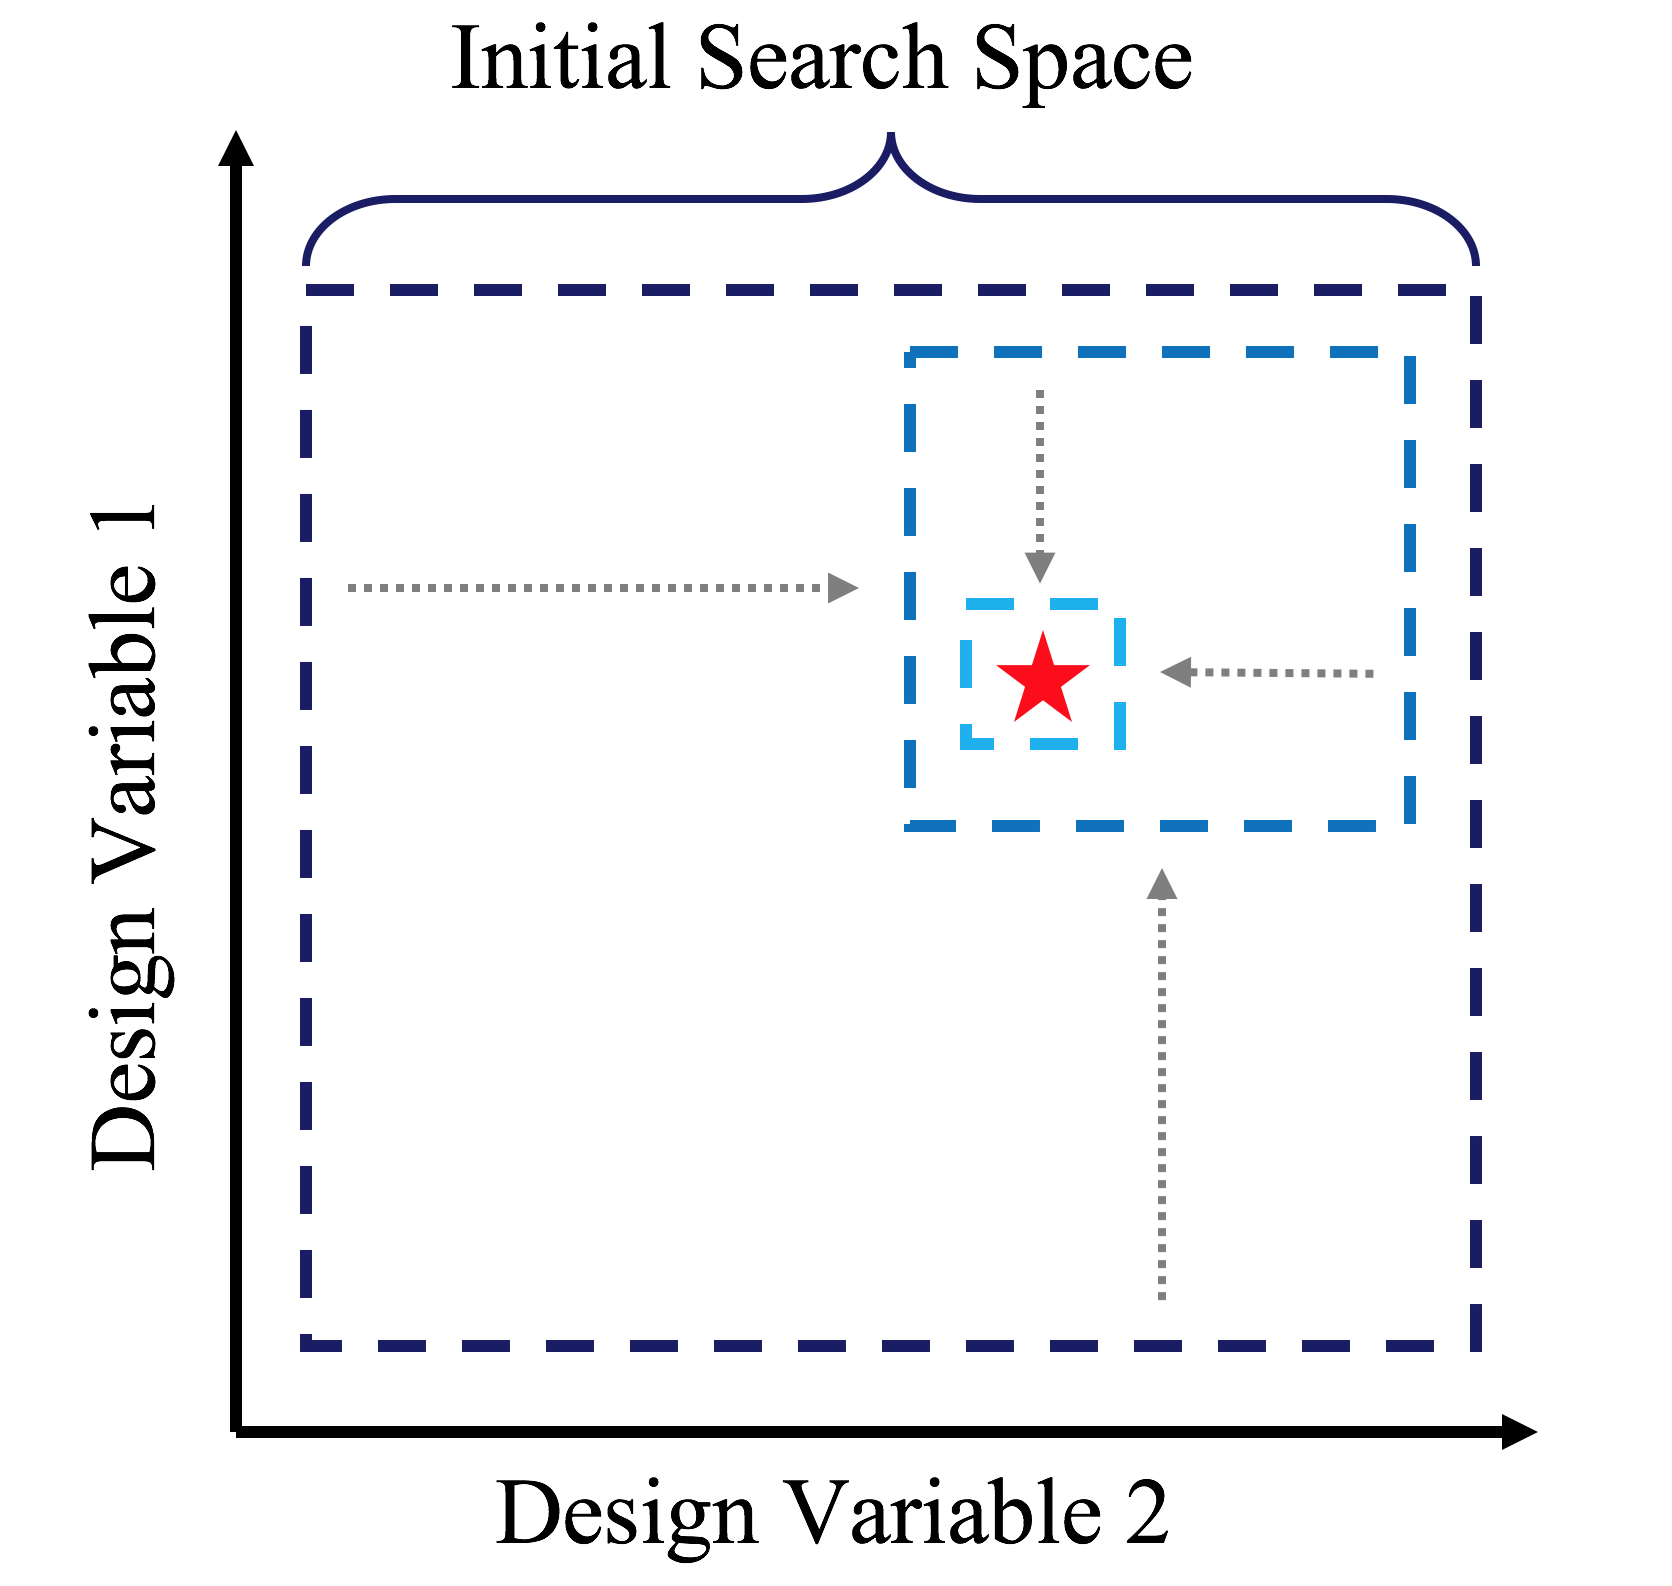
\includegraphics[width=0.7\textwidth]{ParameterSweeps/figures/searchSpace.png}
    \caption{Representation of iteratively narrowing the search space to find an optimal solution}
    \label{fig:searchSpace}
\end{figure}

